\documentclass{article}

% if you need to pass options to natbib, use, e.g.:
\PassOptionsToPackage{numbers, compress}{natbib}
% before loading nips_2018

% ready for submission
\usepackage[final]{nips_2018}

\usepackage{wrapfig}

% to compile a preprint version, e.g., for submission to arXiv, add
% add the [preprint] option:
% \usepackage[preprint]{nips_2018}

% to compile a camera-ready version, add the [final] option, e.g.:
% \usepackage[final]{nips_2018}

% to avoid loading the natbib package, add option nonatbib:
% \usepackage[nonatbib]{nips_2018}

\usepackage[utf8]{inputenc} % allow utf-8 input
\usepackage[T1]{fontenc}    % use 8-bit T1 fonts
\usepackage{hyperref}       % hyperlinks
\usepackage{url}            % simple URL typesetting
\usepackage{booktabs}       % professional-quality tables
\usepackage{amsfonts}       % blackboard math symbols
\usepackage{amsmath}       % blackboard math symbols
\usepackage{amssymb, amsthm}       % blackboard math symbols
\usepackage{nicefrac}       % compact symbols for 1/2, etc.
\usepackage{microtype}      % microtypography
\usepackage{xcolor}
\usepackage{algpseudocode,algorithm,algorithmicx}
\usepackage{comment}
%\usepackage{subfigure}
\usepackage{subcaption}
\usepackage{cleveref}

\usepackage{graphicx}
\graphicspath{{figures/}}

\usepackage{tikz}
\usepackage{pgffor}
\usetikzlibrary{arrows,positioning}

% My commands
\newcommand{\R}{\mathbb{R}}
\newcommand{\N}{\mathbb{N}}
\newcommand{\E}{\mathbb{E}}
\newcommand{\TODO}[1]{\textcolor{red}{\textbf{TODO: #1}}}
%\newcommand{\TODO}[1]{}

\newcommand{\cA}{\mathcal{A}}
\newcommand{\cH}{\mathcal{H}}
\newcommand{\cL}{\mathcal{L}}
\newcommand{\cN}{\mathcal{N}}
\newcommand{\cO}{\mathcal{O}}
\newcommand{\cS}{\mathcal{S}}
\DeclareMathOperator*{\argmax}{argmax}
\DeclareMathOperator*{\maximize}{maximize}
\DeclareMathOperator{\unif}{unif}

\newcommand{\sysid}{dynamics}
\newcommand{\blind}{\emph{blind}}
\newcommand{\plain}{\emph{plain}}
%\newcommand{\extra}{\emph{extra}}
\newcommand{\embed}{\emph{ours}}
\newcommand{\traj}{\emph{traj}}
\newcommand{\embedfn}{e}
\newcommand{\idfn}{id}


\newcommand{\obset}{\mathcal{Z}}
\newcommand{\idset}{\mathcal{D}}
\newcommand{\obvar}{z}
\newcommand{\idvar}{d}
\newcommand{\idpdf}{p_{\idset}}
\newcommand{\latset}{\mathcal{E}}
\newcommand{\latvar}{\varepsilon}

\newcommand{\secref}[1]{Section \ref{#1}}
\newcommand{\figref}[1]{Figure \ref{#1}}
\newcommand{\tabref}[1]{Table \ref{#1}}
\newcommand{\KH}[1]{\textcolor{blue}{ #1}}

\newtheorem{theorem}{Theorem}[section]
\newtheorem{corollary}[theorem]{Corollary}
\newtheorem{lemma}[theorem]{Lemma}
\newtheorem{assumption}[theorem]{Assumption}
\newtheorem{definition}[theorem]{Definition}


\title{Learning a System-ID Embedding Space for Domain Specialization with Deep Reinforcement Learning}

% The \author macro works with any number of authors. There are two
% commands used to separate the names and addresses of multiple
% authors: \And and \AND.
%
% Using \And between authors leaves it to LaTeX to determine where to
% break the lines. Using \AND forces a line break at that point. So,
% if LaTeX puts 3 of 4 authors names on the first line, and the last
% on the second line, try using \AND instead of \And before the third
% author name.

\author{
  James A.~Preiss \\
  %Dep't. of Computer Science\\
  Univ. of Southern California\\
  Los Angeles, CA 90089\\
  \texttt{japreiss@usc.edu}
  %% examples of more authors
  \And
  Karol Hausman \\
  Google Brain \\
  %1600 Amphitheatre Parkway\\
  Mountain View, CA 94043 \\
  \texttt{karolhausman@google.com}
  \And
  Gaurav S. Sukhatme \\
  %Dep't. of Computer Science\\
  Univ. of Southern California\\
  Los Angeles, CA 90089\\
  \texttt{gaurav@usc.edu}
  %% Coauthor \\
  %% Affiliation \\
  %% Address \\
  %% \texttt{email} \\
  %% \And
  %% Coauthor \\
  %% Affiliation \\
  %% Address \\
  %% \texttt{email} \\
  %% \And
  %% Coauthor \\
  %% Affiliation \\
  %% Address \\
  %% \texttt{email} \\
}


\begin{document}

\maketitle

\begin{abstract}
\vspace{-0.1cm}
We propose a method to improve the ability of reinforcement-learned policies to adapt to unknown dynamics of the agent at test time.
Our method learns an embedding space
to distill system identification information into a form that is both useful for policy specialization, and easy to estimate.
%Instead, we propose to to ease the difficulty of system identification by learning an abstract embedding space
%Agents trained with reinforcement learning often fail to generalize to test environments with different dynamics.
%but its effectiveness is limited to scenarios where a policy that is oblivious to \sysid{} parameters is sufficient.
%a unimodal policy is sufficient for all possible test environments.
%For larger variations some form of system identification is needed.
%However, identifying every dynamics parameter accurately can be a difficult -- and unnecessary -- intermediate step to optimal behavior.
%Instead, we propose to to ease the difficulty of system identification by learning an abstract embedding space
%that distills system identification information into a form that is both useful and easier to estimate.
%Our framework also includes an observability-promoting reward that encourages the policy to balance the task goal with behavior that aids system identification.
%Simulation experiments demonstrate improved generalization to novel test environments, and show desirable properties of the learned space.
%Reinforcement learning (RL) is a highly general framework for learning control policies
%ithout per-environment manual effort.
%et, in contrast to the generality of RL itself,
\end{abstract}

\vspace{-0.3cm}
\section{Introduction and related work}
\vspace{-0.2cm}

Policies trained with reinforcement learning (RL) are often brittle and fail to generalize beyond the training environment.
An important instance of this problem is sim-to-real transfer for robotics. %to other environments.
%, even when the differences are small~\citep{zhang-study-on-overfitting}.
%This issue has become the subject of considerable attention from RL researchers.
%Such overfitting to the training environment is problematic as it does not allow to transfer trained policies, e.g. from simulation to reality. Training in a fast simulator and deploying on a real robot can save time,
%but since simulators cannot faithfully reproduce every detail of physical phenomena such as fluid dynamics, contacts or friction forces,
%policies must be able to generalize from the training to the test scenario.
%The problem of overfitting to the training environment is important beyond simulation-to-real transfer;
%for example, it also occurs when deploying a pre-trained policy on a set of robots with manufacturing variations.
%-- e.g., when training a policy in a lab and deploying it on mass-produced robots with manufacturing variations, different wear and tear, etc. that will affect dynamics.
Domain randomization during training can improve robustness~\citep{antonova-pivoting-corr17, zhu-RL-IL-diverse, baar2018simtoreal, sadeghi-cad2rl-rss17, tobin-domainrand-arxiv17},
but it is limited by its assumption that a single policy can perform adequately in all possible test domains.
In addition, domain randomization introduces partial observability to the underlying MDP as the agent is not aware of the changes in its randomized dynamics.
% Related approaches include ensembles of policies~\citep{actor-mimic,teh-distral},
% adversarial perturbations of state or observations~\citep{pinto-robust-adversarial-RL,huang-adversarial-attacks},
% and learning robust feature spaces~\citep{higgins-DARLA,bousmalis-domainseparation-nips16}.
% Fine-tuning\TODO{fine-tuning citation} or progressive networks~\citep{rusu-progressive-nets} 
% use a policy trained in simulation as a starting point for further learning in the test environment.
% Model-agnostic meta-learning (MAML)~\citep{finn-maml-icml17}
% explicitly prepares for the fine-tuning by unrolling the policy gradient update in the training objective.
% \TODO{end this paragraph.}
Meta-learning and fine-tuning~\citep{finn-maml-icml17, rusu-progressive-nets, duan-rl2}
assume there will be an opportunity
to collect data from the test domain and update the policy.
%
%Visual differences between training and a specific test environment have been addressed
%using generative adversarial networks (GANs)~\citep{bousmalis-domain-gan-cvpr17}
%or by learning a feature space that is invariant to differences between the two domains~\citep{bousmalis-domainseparation-nips16}.
%
In this work, we seek a policy that specializes to a novel test environment rapidly,
without using significant data or computational effort at test time.

We assume that \sysid{} parameters are known during training but unknown under test.
Our method includes two key contributions:
1) a learned embedding space that represents the system \sysid{} parameters
in a form that is both useful and easy to identify,
%a learned mapping from system \sysid{} parameters to an abstract embedding space,
%and a corresponding identification function to estimate the embedding value at test time,
and 2) an observability reward that encourages the agent to maximize identification accuracy.
%in addition to the primary task.
We eliminate the task of
estimating the actual \sysid{} parameters of the test environment,
as in~\citep{yu-up-osi-rss17},
without introducing the training complexity of a recurrent policy as in~\citep{peng-dynamics-randomization-corr17}.
%We demonstrate experimentally that our learned embeddings have desirable properties,
%and reduce generalization error at test time.


\vspace{-0.2cm}
\section{Problem statement and method}
\label{problem-method}
\vspace{-0.2cm}

We consider RL in a continuous Markov decision process
%where $\cS \subseteq \R^\cS$ is the state space,
%$\cA \subseteq \R^\cA$ is the action space,
%$p : \cS \times \cA \times \cS \mapsto \R_{\geq 0}$ are the stochastic dynamics,
%$\rho : \cS \mapsto \R_{\geq 0}$ is the initial state distribution,
%and $r : \cS \times \cA \mapsto \R$ is the task reward function.
with states $\cS \subseteq \R^n$,
actions $\cA \subseteq \R^d$,
dynamics $p : \cS \times \cA \times \cS \mapsto \R_{\geq 0}$,
%stochastic dynamics $p(s_{t + 1} | s_t, a_t)$,
initial state distribution $\rho : \cS \mapsto \R_{\geq 0}$,
and rewards $r : \cS \times \cA \mapsto \R$.
%and finite horizon $H \in \mathbb{N}$.
%~\TODO{explicitly use probability measures or density functions here, instead of functions to $\R_{\geq 0}$?}
%
The state $\cS$ is partitioned into
an \emph{observed space} $\obset$
consisting of the changing states such as angles and angular velocities of joints,
and a \emph{\sysid{} space} $\idset$
%consisting of parameters such as
consisting of joint geometries, moments of inertia, coefficients of friction, etc.
%such that $\cS = \obset \times \idset$.
%These states can be measured or accurately estimated in the real system.
During training, $\idvar \in \idset$ is known, %the full state space $\obset \times \idset = \cS$,
but at test time the agent only observes $\obvar \in \obset$.
%The \sysid{} parameters follow the distribution $\idpdf(\idvar) : \idset \mapsto \R_{\geq 0}$.
Our goal is to learn a policy $\pi$ %: \obset \times \idset \times \cA \mapsto \R_{\geq 0}$
that maximizes a standard RL objective in expectation over a distribution $\idpdf$ on $\idset$.
%\begin{equation}\begin{split}
%\pi : \cS \times \cA \mapsto \R_{\geq 0}, \quad
%\pi^\star = \argmax_\pi\ J_R(\pi) \triangleq \E_{\idvar \sim \idpdf,\ \tau \sim p(\tau|\pi,\idvar)} \sum_{t = 0}^H
%r(s_t, a_t),
%\label{objective}
%\end{split}\end{equation}
%where $\tau = (s_0, a_0), \dots, (s_H, a_H)$ denotes a state-action trajectory and
%, with a slight abuse of notation, 
%$p(\tau | \pi, \idvar)$ denotes the trajectory distribution induced by $\pi$ under \sysid{} parameters $\idvar$.
%\begin{equation}\begin{split}
%p(\tau | \pi, \idvar) = \rho(s_0) \prod_{t=0}^{H-1} p(s_{t+1} | s_t, a_t) \pi(a_t|\obvar_t, \idvar_t).
%\end{split}\end{equation}
%~\TODO{add discount?}
If $\idpdf$ covers a wide enough range of system dynamics,
it is reasonable to assume that no \blind{} policy,
where $\pi(a|\obvar,\idvar) = \pi(a|\obvar)\ \forall\ \idvar \in \idset$,
can perform adequately.
%is acceptably close to maximizing~\eqref{objective}.

A natural approach is to train a policy $\pi(a|\obvar,\idvar)$ conditioned on the known value of $\idvar$,
alongside a \emph{system identification} function that yields an estimate $\delta$ of $\idvar$.
At test time, we act with the policy $a \sim \pi(a|\obvar, \delta)$.
This method, explored by~\citet{yu-up-osi-rss17}, creates two challenges.
First, it requires estimating every \sysid{} parameter,
even though some may be difficult to estimate, redundant, or unneeded to maximize reward. %~\eqref{objective}.
%An example of this issue is shown in the experiment of \secref{pointmass}.
%where a mass and an actuator power are reduced to a single dimensionless quantity.
%Reductions such as these can make the system identification problem easier, but they may not be easy to derive by hand on complex systems.
Second, behavior that maximizes reward % the expected reward~\eqref{objective}
in training may be suboptimal for system identification.
%in training with known $\idvar$ may not be the best behavior for making the system identification task easier.
It is preferable to learn a behavior that balances the primary reward %~\eqref{objective}
with a secondary goal of making the system identification task as easy as possible. %so that the agent can quickly identify how it should specialize its behavior.

%\subsection{Embedding \sysid{} space}
We address both of these concerns by introducing
a learned abstract representation
$\latset \subseteq \R^{d_\latset}$
of the \sysid{} parameters.
This creates an opportunity to distill the full complexity of $\idset$
into a form that is potentially more useful for the policy to produce optimal behavior,
while simultaneously being easier to estimate.
During training, we learn an embedding function $\embedfn : \idset \mapsto \latset$
and a policy $\pi_\latvar(a|s,\latvar)$, where $\latvar = \embedfn(\idvar)$.
We simultaneously learn an identification function $\idfn : (\obset \times \cA)^K \mapsto \latset$,
to estimate the embedding value from a fixed-length state-action trajectory.
To aid observability, we augment the main RL reward with a term penalizing estimation error of $\idfn$,
thus rewarding behavior that makes estimating $\latvar$ easier.
%The embedding space dimensionality $d_\latset$ and the window length $1 \leq K \ll H$ are user-chosen hyperparameters.
%The functions $\embedfn$ and $\idfn$ are learned simultaneously with the policy $\pi$ in an end-to-end fashion.
%The training and test setup follow the scenario described at the beginning of this section.
Then, at test time, we store a rolling buffer $\tau$ of the past $K$ pairs $(\obvar,a)$
and act with the policy $a_t \sim \pi_\latvar(a_t|\obvar_t, \idfn(\tau_{t-K:t}))$.

%\TODO{possibly mention observability.}

\begin{comment}
While the embedding space may help make system identification easier,
it has a failure mode that must be considered:
if $\embedfn$ and $\idfn$ both map to the same constant value for any input,
$\idfn$ will achieve perfect performance during training,
but the embedding will not influence the policy, and $\pi_\latvar$ will be reduced to a \blind{} policy
equivalent to that learned under pure domain randomization.
To avoid this problem, we impose a structure where the parameters of the embedding function $e$
can only be learned via backpropagation of the RL objective gradient through $\pi_\latvar$.
We then augment the main objective~\eqref{objective} with an \emph{observability objective} term
rewarding accurate system identification of $\latvar$:
\begin{equation}\begin{split}
J_{\idfn}(\pi_\latvar, \embedfn) =
-\E_{\idvar \sim \idpdf,\ \tau \sim p(\tau|\pi_\latvar,\idvar)}
\left[
\sum_{t = 0}^{H} \| \idfn(\tau_{t-K:t}) - \embedfn(\idvar) \|_2^2
%+ \alpha_{id} \E_{\tau \sim \text{\TODO{complicated}}} \| id(\tau) - e(s_d) \|_2 \\
\right],
%&+ \alpha_{KL} KL(e(s_d), \cN(0,1))
\label{objective-observability}
\end{split}\end{equation}
where $\tau_{t-K:t}$ denotes the $K$-length sub-trajectory of $\tau$ ending at time $t$.
We additionally include an entropy regularization term,
\begin{equation}\begin{split}
J_{\cH}(\pi_\latvar) =
\E_{\idvar \sim \idpdf,\ \tau \sim p(\tau|\pi_\latvar,\idvar)}
\cH(\pi_\latvar(\cdot |\obvar, \idvar)),
\label{objective-entropy}
\end{split}\end{equation}
because it is inherent in the Soft Actor-Critic (SAC) RL algorithm~\citep{haarnoja-soft-actor-critic} we use in experiments.
\TODO{this is PPO fake entropy, not SAC real entropy.}
\TODO{say more about choice of RL algorithm, why entropy is probably especially good for us.}
The complete RL objective is given by
\begin{equation}\begin{split}
J(\pi_\latvar, \embedfn) = J_R(\pi) + \alpha_{id} J_{\idfn}(\pi, \embedfn) + \alpha_{\cH} J_{\cH}(\pi).
\label{objective-full}
\end{split}\end{equation}
\TODO{talk about reward scaling in SAC? really, there is no $\alpha_{\cH}$.}
The regularization weights $\alpha_{id} > 0,\ \alpha_{\cH} > 0$ are user-chosen hyperparameters.

Note that the summation in~\eqref{objective-observability} intentionally includes negative values of the timestep $t$.
At test time, $\idfn$ will be required to produce an input to $\pi_\latvar$
before enough time has passed to fill the $K$-length history buffer.
We thus initialize this buffer with zeros, and include a reward for these initial timesteps in~\eqref{objective-observability}.
The value of states and actions for negative values of $t$ are defined as zero.

We emphasize that the observability objective term~\eqref{objective-observability}
is added to the reinforcement learning reward rather than optimized directly.
The parameters of $\idfn$ are considered constant when optimizing $\pi_\latvar$ and $e$;
and the parameters of $\embedfn$ are considered constant when optimizing $\idfn$.
The reward $r_{\idfn}$ of the action $a_t$ includes the system identification accuracy
of all $K$-windows containing $t$, as follows:
\begin{equation}\begin{split}
r_{\idfn}(s_t, a_t) = \frac{1}{K}
\sum_{t' = t - K + 1}^t
\| \idfn(\tau_{t':t'+K}) - \embedfn(s_d) \|_2^2
\label{sysid-reward}
\end{split}\end{equation}
where the error is defined as zero for out-of-bound windows.
%and a KL divergence term encouraging the distribution of the embeddings
%to match the first two moments of the unit normal distribution.
%The latter ensures that the supervised learning data sets presented to the identification function $id$ do not require any separate whitening step.
%\TODO{better motivation? It also helps avoid the collapse to a constant function,
%but technically we already ``solve'' that by adding the estimation loss to the RL objective...}
The system identification function $\idfn$ is not updated by the RL algorithm.
It is updated in a separate supervised learning step, performed alongside each iteration of RL.
%In addition, we add fixed Gaussian noise to the output of $\embedfn$ using the reparameterization trick; this encourages robustness against small errors in system identification at test time.

\end{comment}




\begin{comment}
\begin{table}[ht]
\centering
\begin{tabular}{lll}
Type     & Filters & Size \\
\hline
Input    & --           & dim($\cS \times \cA$) \\
Conv1D   & 32           & 3 \\
Conv1D   & 32           & 3 \\
ReLu     & --           & -- \\
Max Pool & --           & 2 \\
Conv1D   & 32           & 5 \\
ReLu     & --           & -- \\
Linear   & dim($\latset$)   & -- \\
\end{tabular}
\caption{Architecture of 1D convolutional neural network used to learn the embedding identifier $id$.}
\label{conv1d}
\end{table}
\end{comment}




\vspace{-0.2cm}
\section{Experiments}
\vspace{-0.2cm}

In this section, we show desirable properties of our learned embedding space $\latset$
and compare the performance of our architecture against several baselines.
%The domain randomization policy with no access to $\idvar$ is denoted as \blind{}.
%The policy conditioned on the true system identification parameters $\idvar$ instead of the learned embedding,
%similar to~\citet{yu-up-osi-rss17}, is denoted by \plain{}.
Details are given in~\Cref{appendix-exp}.

%The presented experimental results suggest that our embedding framework learns policies that generalize better than the alternatives \TODO{fingers crossed.}

%\subsection{Point-Mass Environment}
\textbf{Point-Mass Environment:}
\label{pointmass}
This low-dimensional system allows us to visualize learned embeddings.
A 2D point mass $p \in \R^2$ follows dynamics $\ddot p = a$ for action $a \in [-1,1]^2$ and reward $r = -\|p\|_2$.
%The observed state 
%$\obvar = (p \in \R^2, v \in \R^2)$
%is position and velocity of the unit mass in 2D.
The system identification state $\idvar$ is a gain factor $g \in \pm[0.175, 1.75]$,
such that the true force applied to the mass is $g \cdot a$.
%The system dynamics are
%$\dot p = v, \quad \dot v = -f v + ga$,
%where $0 < f \ll 1$ is a fixed friction parameter.
%by the reward function $r = -\sqrt{|g|} \cdot \|p\|_1$,
%where the scaling factor $\sqrt{|g|}$ balances the rewards in the low- and high-gain scenarios
%based on the minimum-time bang-bang solution to the implied optimal control problem.
Due to the unknown sign of $g$, a domain randomization policy cannot possibly perform well in this environment.
%However, since the gain parameter $g$ is trivial to estimate, there is no reward difference between \embed{} and \plain{}.
%\TODO{better explanation, avoid readers thinking it's too contrived}
%
%The point-mass learning curves are shown in \TODO{figure}.
%As expected, the \emph{blind} policy performs very poorly.
%The \emph{plain} and \emph{extra} policies perform in between.
%
\begin{comment}
\begin{table}
\centering
\begin{tabular}{l c c c c}
       &          & test         & reward $\sigma$          & reward $\sigma$       \\
flavor & $\alpha$ & reward $\mu$ &            (per-episode) &            (per-seed) \\
\hline
\blind & N/A & -80.3 & 27.6 & 2.6 \\
\plain & 0.1 & -70.8 & 28.2 & 2.4 \\
\extra & 0.1 & -67.1 & 34.6 & 2.7 \\
\embed & 0.1 & \textbf{-62.7} & 27.6 & 0.8 \\
\end{tabular}
\end{table}
\end{comment}
%
\begin{figure}
    \centering
    \begin{subfigure}[b]{0.24\textwidth}
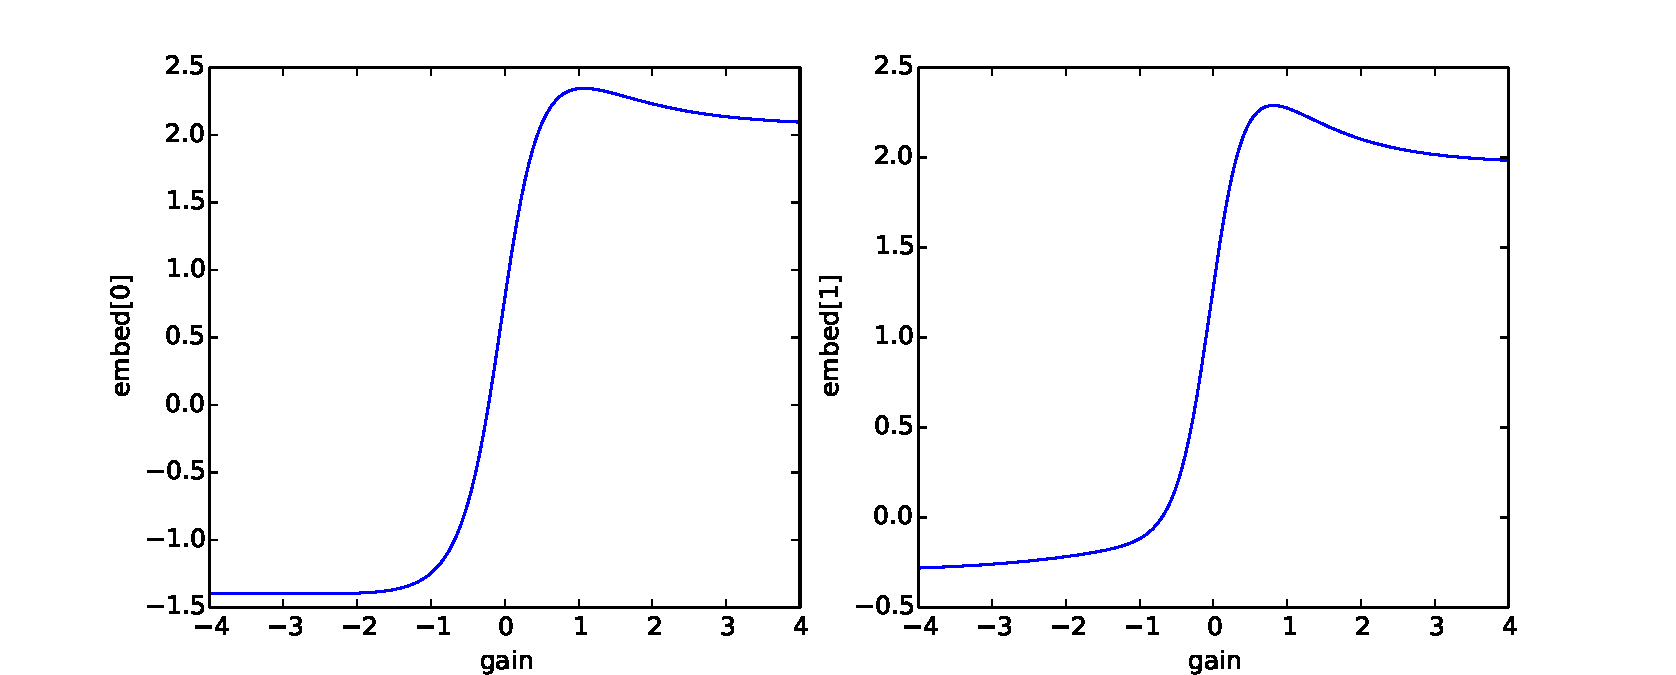
\includegraphics[trim={13.7cm -1cm 2cm -1.0cm}, clip, width=\textwidth]{pointmass_embed_mapping.pdf}
        \caption{Learned mapping from gain $g$ to one dimension of embedding space $\latset$.
        }
        \label{embed-mapping}
    \end{subfigure}
    ~ %add desired spacing between images, e. g. ~, \quad, \qquad, \hfill etc. 
      %(or a blank line to force the subfigure onto a new line)
    \begin{subfigure}[b]{0.48\textwidth}
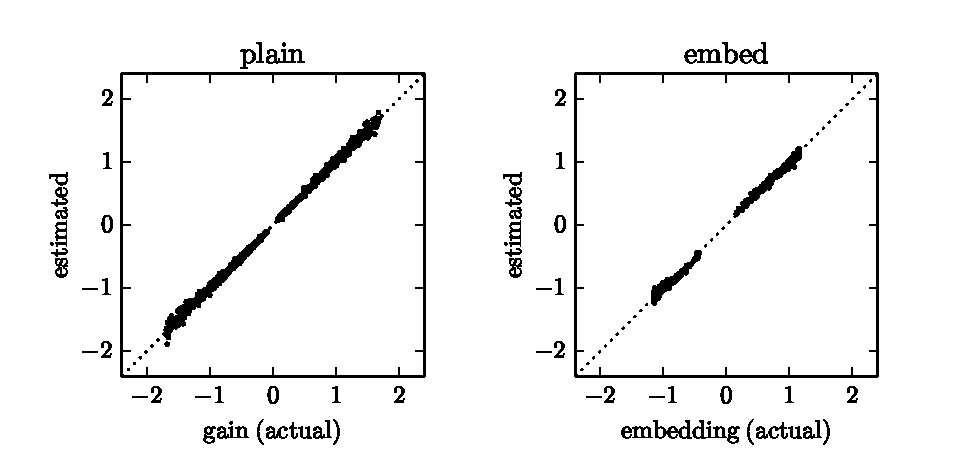
\includegraphics[trim={0.5cm 0 1cm 1.2cm}, clip, width=\textwidth]{pointmass_embed_scatter.pdf}
        \caption{
Comparison of actual vs. estimated gain $g$ (left) and embeddings $\latset$ (right).
Embedding spreads parameters requiring disjoint behavior to distant clusters.
        }
        \label{embed-scatter}
    \end{subfigure}
    ~ %add desired spacing between images, e. g. ~, \quad, \qquad, \hfill etc. 
    %(or a blank line to force the subfigure onto a new line)
    \begin{subfigure}[b]{0.23\textwidth}
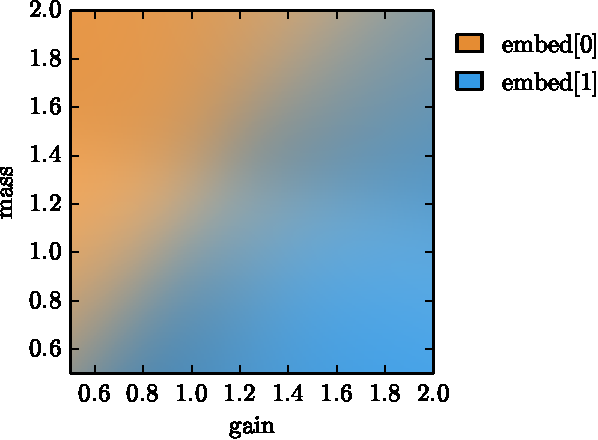
\includegraphics[trim={0 0 2.5cm 0}, clip, width=\textwidth]{embed_colors.pdf}
        \caption{
With redundant parameters,
%Graph axes represent true dynamics parameters; each color represents one dimension of the learned 2D embedding.
%In point-mass environment with parameters of gain $g$ and mass $m$,
%the dynamics only depend on the $g/m$ ratio.
$g=m$ line (spatial) maps to same $\latvar$ (color).
%The learned embedding reflects this; for example, the $g=m$ line is all mapped to similar embedding values.
%Plot restricted to positive gain domain for clarity.
}
        \label{fig:embed_colors}
    \end{subfigure}
    \caption{
    Desirable properties of learned embedding $\embedfn : \idset \mapsto \latset$ for point-mass environment.
    }
\vspace{-0.4cm}
\end{figure}
%
\begin{comment}
\begin{figure}
\centering
\caption{
\emph{Left}:
\emph{Middle}: Actual vs. estimated gain parameter $g$ for \plain{} policy.
\emph{Right:} Actual vs. estimated learned embedding in $\latset$ with \embed{} policy (one of two dimensions).
}
\caption{
}
\label{fig:embed_colors}
\end{figure}
\label{embed-mapping}
\end{figure}
\end{comment}
%
As shown in~\Cref{embed-mapping,embed-scatter},
%illustrate the mapping %$\embedfn$ from $g$ to the embedding space $\latset$.
%The scatter plots compare the ground truth embedding values
%against those estimated by $\idfn$ in the \embed{} policy,
%and the ground truth gain factor $g$ against the values estimated by the equivalent of $\idfn$ in the \plain{} policy.
%Against the $x-$axis, density estimates are shown.
the learned $\embedfn$ ``squashes'' the gain factor $g$ into positive and negative clusters,
helping the policy switch between disjoint behavior styles.
%The clustering creates an easier enput for the policy to switch between disjoint behavior styles. % depending on the sign of the gain factor.
%The ``squashing'' does not impede the task reward of the policy,
%since an identical bang-bang control policy is optimal for any magnitude of $g$ -- only the sign of the input needs to change.

To demonstrate distillation of redundant parameters, %our approach's ability to distill dynamics parameters,
%into a simplified space where only the information needed to achieve good rewards is preserved.
%We illustrate this by constructing a version of the point-mass environment with redundant features:
we construct a version of the point-mass environment with a mass parameter $m$ alongside the gain $g$, such that $\ddot p = ga/m$,
making all $(g, m)$ combinations with the same ratio indistinguishable. % to system identification.
%This poses a problem for the \plain{} 
%or \extra{} frameworks
%framework
%because the learning problem of recovering the true $(g, m)$ from a state-action trajectory is ill-posed.
This poses a problem for any approach that requires accurate identification of $\idset$ at test time.
In contrast, our framework learns an embedding where all $(g, m)$ combinations with similar ratios map similar embedding values,
as shown in~\Cref{fig:embed_colors}.

\begin{comment}
\begin{figure}
\centering
\TODO{learning curves for redundant point-mass.}
\caption{
Example of incompatibility between our observability objective \TODO{ref}
and attempting to reconstruct the true dynamics parameters
in redundant point-mass environment.
When $\alpha = 0.1$, \extra{} network alters its behavior in pursuit of the observability reward, but the dynamics parameters are impossible to identify.
The learning process is disturbed.
When $\alpha = 0$, \extra{} network does not alter its behavior
and learns a policy that accounts for the many-to-many characteristic of the system identification problem.
}
\label{fig:redundant_fail}

\end{figure}
\end{comment}

%\subsection{Half-Cheetah Environment}

\textbf{Half-Cheetah Environment:}
As a more complex task, we demonstrate results on the \emph{Half-Cheetah}
planar locomotion environment from the OpenAI Gym~\citep{openai-gym}.
%The following parameters are randomized:
%We randomize thelengths of all kinematic links, damping, stiffness, and ranges of all revolute joints, and gear ratios of all actuators.
We randomize 37 kinematic and dynamic parameters of the model (see~\Cref{appendix-exp} for details).
%In total, 37 parameters are randomized.
The embedding space $\latset$ is 8-dimensional; we did not observe significant sensitivity to this choice.
%Each end of the joint range is shifted by $\pm 0.3$ radians.
%All other parameters are multiplied by a ratio log-uniformly distributed in the range $[\beta^{-1}, \beta]$ with $\beta = 1.75$.
%\TODO{describe these perturbations more precisely}

%Due to the architecture of the MuJoCo physics simulator used in this environment~\citep{todorov-mujoco},
%it is not practical to sample new random dynamics parameters $\idvar$ for each training iteration.
%Instead, we train on a fixed set of 256 randomized models.
%At test time, we sample a new, independent set of 256 randomized models.
%Instead, we construct a ``universe'' of 256 models initially, and randomly choose 8 of these environments for each training iteration.
%At test time, we resample a new ``universe'' of models.
\begin{wrapfigure}{r}{0.45\textwidth}
    \vspace{-0.75cm}
    \centering
    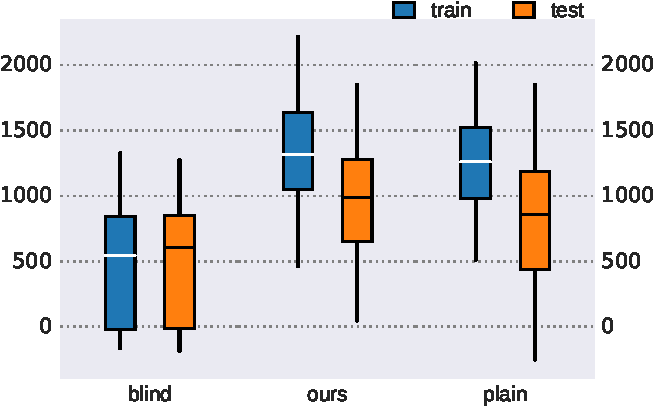
\includegraphics[width=0.4245\textwidth]{lastmain-crop.pdf}
    \caption{Box plot of training and test reward for \blind{}, \embed{}, and \plain{} policies.
    Whiskers indicate full extent (min/max) of rewards.}
    \label{cheetah-box}
\end{wrapfigure}

Results are shown in~\Cref{cheetah-box}.
Variance of rewards is large due to the randomized dynamics.
The \blind{} policy fails to achieve high rewards because it is unable to specialize its behavior to the \sysid{} parameters.
The \plain{} policy, conditioned on $\idvar$ instead of $\latvar$, achieves similar training rewards but worse generalization error,
and suffers negative rewards in some test environments, while \embed{} does not.

In current experiments, we have not yet observed a significant effect of our observability reward term.
In future work, we plan to investigate other systems where observability-seeking behavior is most critical.

\paragraph{}
\vspace*{-\parskip}

%The data show that, while the \plain{} policy performs slightly better in training,
%it suffers from worse generalization error.
%The \embed{} policies achieves lower generalization error and higher test rewards.
%Note that the training, as well as the test, performance for nonzero $\alpha$
%is better for both \embed{} and \plain{} policies.
%We hypothesize that behaving the same for all $\idvar$ values, like the \blind{} policy,
%is a local optimum in the policy space,
%whereas the optimal policy specializes for each $\idvar$,
%but this optimum is more difficult to find.
%The observability reward provides an additional incentive
%for the policy to behave differently for environments with different $\idvar$ values,
%pulling it away from the undesirable local optimum.

\bibliographystyle{plainnat}
\bibliography{bibliography}{}

\newpage
\appendix

\section{Expanded description of method}

In this section, we give additional details on our proposed method outlined in~\Cref{problem-method}.
As previously mentioned, we operate in the continuous MDP defined by $(\cS, \cA, p, \rho, r)$.
We partition the state space $\cS$ into observed states $\obset$ and dynamics states $\idset$.
To aid exposition, we refer to the full state $s$ and the pair $(\obvar, \idvar)$ interchangeably as appropriate.
%These states can be measured or accurately estimated in the real system.
The states in $\idset$ influence the system dynamics, i.e.
\begin{equation}
\idvar_1, \idvar_2 \in \idset,\ \idvar_1 \neq \idvar_2 \implies p(s|a,\obvar,\idvar_1) \neq p(s|a,\obvar,\idvar_2)
\end{equation}
for $s \in \cS,\ a \in \cA,\ \obvar \in \obset$ in general,
but $\idvar$ is unobserved by the agent at test time.
This setting could also be formalized as a partially observable MDP (POMDP),
but we use the present formalism to emphasize the following assumptions:
\begin{assumption}
The dynamics state $d$ is independent of the observed states and actions:
\[
p(\idvar_{t+1}|a_t, \obvar_t, \idvar_t) = p(\idvar_{t+1}).
\]
\end{assumption}
In this paper, we consider episodic RL and hold $\idvar$ constant during a single episode;
however, our architecture does not prohibit training under non-stationary $\idvar$ and in non-episodic environments.
\begin{assumption}
The test-time observation is a deterministic truncated identity function $O(\obvar, \idvar) = \obvar$,
rather than a more general and/or stochastic function.
\label{observation}
\end{assumption}
This assumption emphasizes that we are not concerned with the partial observability resulting from, e.g.,
an agent perceiving its environment through a camera.

In training, the \sysid{} parameters follow the distribution $\idpdf(\idvar) : \idset \mapsto \R_{\geq 0}$.
We note that in practical applications, we are often free to choose $\idpdf$,
in which case we should choose a distribution that covers all values of $\idvar$ that might be encountered at test time.
Our goal is to learn the embedding function $\embedfn: \idvar \mapsto \latvar$
and a policy conditioned on the learned embedding $\pi_\latvar: \obset \times \latset \times \cA \mapsto \R_{\geq 0}$
that maximizes the expectation of a standard RL objective over $\idpdf$:
\begin{equation}\begin{split}
%\pi : \cS \times \cA \mapsto \R_{\geq 0}, \quad
\maximize_{\pi,\ \embedfn}\ J_R(\pi_\latvar, \embedfn) \triangleq \E_{\idvar \sim \idpdf,\ \tau \sim p(\tau|\pi_\latvar,\embedfn,\idvar)} \sum_{t = 0}^H
r(s_t, a_t),
\label{objective}
\end{split}\end{equation}
where $\tau = (s_0, a_0), \dots, (s_H, a_H)$ denotes a state-action trajectory and
$p(\tau | \pi_\latvar, \embedfn, \idvar)$ denotes the trajectory distribution induced by $\pi_\latvar$ and $\embedfn$ under \sysid{} parameters $\idvar$:
\begin{equation}\begin{split}
p(\tau | \pi_\latvar, \idvar) = \rho(s_0) \prod_{t=0}^{H-1} p(s_{t+1} | s_t, a_t) \pi_\latvar(a_t|\obvar_t, \embedfn(\idvar_t)).
\end{split}\end{equation}
%~\TODO{add discount?}
%If $\idpdf(\idvar)$ represents only a small region of uncertainty around a fixed system,
%it may be feasible to treat the variation in dynamics caused by $\idvar$
%as an unmodeled source of stochasticity.
%We refer to this approach -- where
%$\pi(a|\obvar,\idvar) = \pi(a|\obvar)$ for all $\idvar \in \idset$ --
%as a \blind{} policy.
%However, we are interested in learning policies that can behave robustly even when the distribution of $d$
%spans a range that is too large to be ignored.
%In other words, we assume:
%\begin{assumption}
%No \blind{} policy $\pi(a|\obvar,\idvar) = \pi(a|\obvar)$
%is acceptably close to maximizing~\eqref{objective}.
%\label{noblind}
%\end{assumption}
%This implies that there exists an observed state $\obvar$ and \sysid{} states $\idvar_i, \idvar_j$
%such that no distribution $\pi(a|\obvar)$ over actions can lead to high rewards
%in both the $\idvar = \idvar_i$ and $\idvar = \idvar_j$ cases.
%If such a condition is possible, then the RL framework must support non-blind policies.
%Our experiments give examples of systems satisfying assumption~\ref{noblind}.
%The combination of assumptions \ref{observation} and \ref{noblind} is the main source of difficulty considered in this paper.
%To make the problem tractable, we assume the availability of a simulator with known \sysid{} parameters for training:
%\begin{assumption}
%The true value of the \sysid{} parameters $\idvar \in \idset$ is known during training, but unknown during testing.
%\label{known-unknown}
%\end{assumption}
%It is important to note that the \sysid{} parameter distribution $\idpdf$ is not an inherent property of the MDP,
%but rather is chosen by us for the training process.
%It should be chosen such that any value of $\idvar$ that can plausibly occur at test time has significant support in $\idpdf$.
%Thus, our setting becomes a fully observable MDP \emph{only} during training time.
%In the following section, we describe our approach to this problem
%and contrast it to existing methods in the literature.
%In the following section, we briefly describe an existing approach to this problem,
%and then introduce the learned system identification embedding that is the main contribution of this work.
%Due to the complexity and nonlinearity of real-world dynamics,
%small errors in the measurements of these states can result in major differences between the behavior of the system in reality and in simulation.
We simultaneously train the identification function $\idfn$ to minimize estimation error
under the induced trajectory distribution:
%$trajectories induced by $\idpdf$ and $\pi$:
\begin{equation}\begin{split}
J_{\idfn}(\idfn, \pi_\latvar, \embedfn) \triangleq
\E_{\idvar \sim \idpdf,\ \tau \sim p(\tau|\pi_\latvar, \embedfn, \idvar)}
\left[
\sum_{t = 0}^{H} \| \idfn(\tau_{t-K:t}) - \embedfn(\idvar) \|_2^2
%+ \alpha_{id} \E_{\tau \sim \text{\TODO{complicated}}} \| id(\tau) - e(s_d) \|_2 \\
\right],
%&+ \alpha_{KL} KL(e(s_d), \cN(0,1))
\label{objective-observability}
\end{split}\end{equation}


While the embedding space may help make system identification easier,
it has a failure mode that must be considered:
if $\embedfn$ and $\idfn$ both map to the same constant value for any input,
$\idfn$ will achieve perfect performance during training,
but the embedding will not influence the policy, and $\pi_\latvar$ will be reduced to a \blind{} policy
equivalent to that learned under pure domain randomization.
To avoid this problem, we impose a structure where the parameters of the embedding function $e$
can only be learned via backpropagation of the RL objective gradient through $\pi_\latvar$.
We then augment the main objective~\eqref{objective} with an \emph{observability objective} term based on $J_{\idfn}$
to reward accurate system identification of $\latvar$.
%: .
%where $\tau_{t-K:t}$ denotes the $K$-length subtrajectory of $\tau$ ending at time $t$.
We additionally include an entropy regularization term,
\begin{equation}\begin{split}
J_{\cH}(\pi_\latvar, \embedfn) \triangleq \E_{\idvar \sim \idpdf,\ \tau \sim p(\tau|\pi_\latvar,\embedfn,\idvar)}
\cH
\left[
\pi_\latvar(\cdot |\obvar, \embedfn(\idvar))
\right],
\label{objective-entropy}
\end{split}\end{equation}
because it is inherent in the Soft Actor-Critic (SAC) RL algorithm~\citep{haarnoja-soft-actor-critic} we use in experiments (additional details in~\Cref{appendix-exp}).
The complete RL maximization objective is given by
\begin{equation}\begin{split}
J(\pi_\latvar, \embedfn) = J_R(\pi_\latvar, \embedfn) - \alpha_{id} J_{\idfn}(\idfn, \pi, \embedfn) + \alpha_{\cH} J_{\cH}(\pi_\latvar, \embedfn).
\label{objective-full}
\end{split}\end{equation}
The regularization weights $\alpha_{id} > 0,\ \alpha_{\cH} > 0$ are user-chosen hyperparameters.
Note that the summation in~\eqref{objective-observability} intentionally includes negative values of the timestep $t$.
At test time, $\idfn$ will be required to produce an input to $\pi_\latvar$
before enough time has passed to fill the $K$-length history buffer.
To include this case in training, we initialize the history buffer with zeros at the episode start (or clear it periodically during non-episodic training),
and include a reward for these initial timesteps in~\eqref{objective-observability}.
The value of states and actions for negative values of $t$ are therefore defined as zero vectors.

We emphasize that the observability objective term~\eqref{objective-observability}
is added to the reinforcement learning reward rather than optimized directly.
The parameters of $\idfn$ are considered constant when optimizing $\pi_\latvar$ and $e$;
and the parameters of $\embedfn$ are considered constant when optimizing $\idfn$.
\begin{comment}
The reward $r_{\idfn}$ of the action $a_t$ includes the system identification accuracy
of all $K$-windows containing $t$, as follows:
\begin{equation}\begin{split}
r_{\idfn}(s_t, a_t) = \frac{1}{K}
\sum_{t' = t - K + 1}^t
\| \idfn(\tau_{t':t'+K}) - \embedfn(s_d) \|_2^2
\label{sysid-reward}
\end{split}\end{equation}
where the error is defined as zero for out-of-bound windows.
\end{comment}
%and a KL divergence term encouraging the distribution of the embeddings
%to match the first two moments of the unit normal distribution.
%The latter ensures that the supervised learning data sets presented to the identification function $id$ do not require any separate whitening step.
%\TODO{better motivation? It also helps avoid the collapse to a constant function,
%but technically we already ``solve'' that by adding the estimation loss to the RL objective...}
The system identification function $\idfn$ is not updated by the RL algorithm.
It is updated in a separate supervised learning step, performed alongside each iteration of RL.
%In addition, we add fixed Gaussian noise to the output of $\embedfn$ using the reparameterization trick; this encourages robustness against small errors in system identification at test time.




\begin{comment}
\begin{algorithm}[h]
\caption{Embed to Identify (E2ID)}
\begin{algorithmic}
\For{\text{\emph{fixed number of iterations}}}
  \State sample dynamics parameters $\idvar^1,\ \dots,\ \idvar^N$ uniformly from $\idset$
  \State collect trajectories $\tau^1,\ \dots,\ \tau^N$ and task rewards from $\pi_\latvar$ for each of the $N$ parameters
  \State evaluate $\idfn$ to estimate embedding $\hat e_D$ for sliding $k-$window over each $\tau$
  \State compute $r_{\idfn}$ according to \eqref{sysid-reward} and add to task rewards $r(s_t,a_t)$
  \State \TODO{off-policy?} update $\pi_\latvar$ using on-policy RL for total reward $J(\pi_\latvar)$ \eqref{objective-full}
  % $r = r_T + \alpha_{\cH}\cH(\pi) + \alpha_{ID} \E_{\pi} (\hat e_D - e_D(s_D))^2$
  \State update system identification network $\idfn$ using supervised learning
\EndFor
\end{algorithmic}
\label{algo}
\end{algorithm}
\end{comment}

\begin{comment}
\begin{figure}
\centering
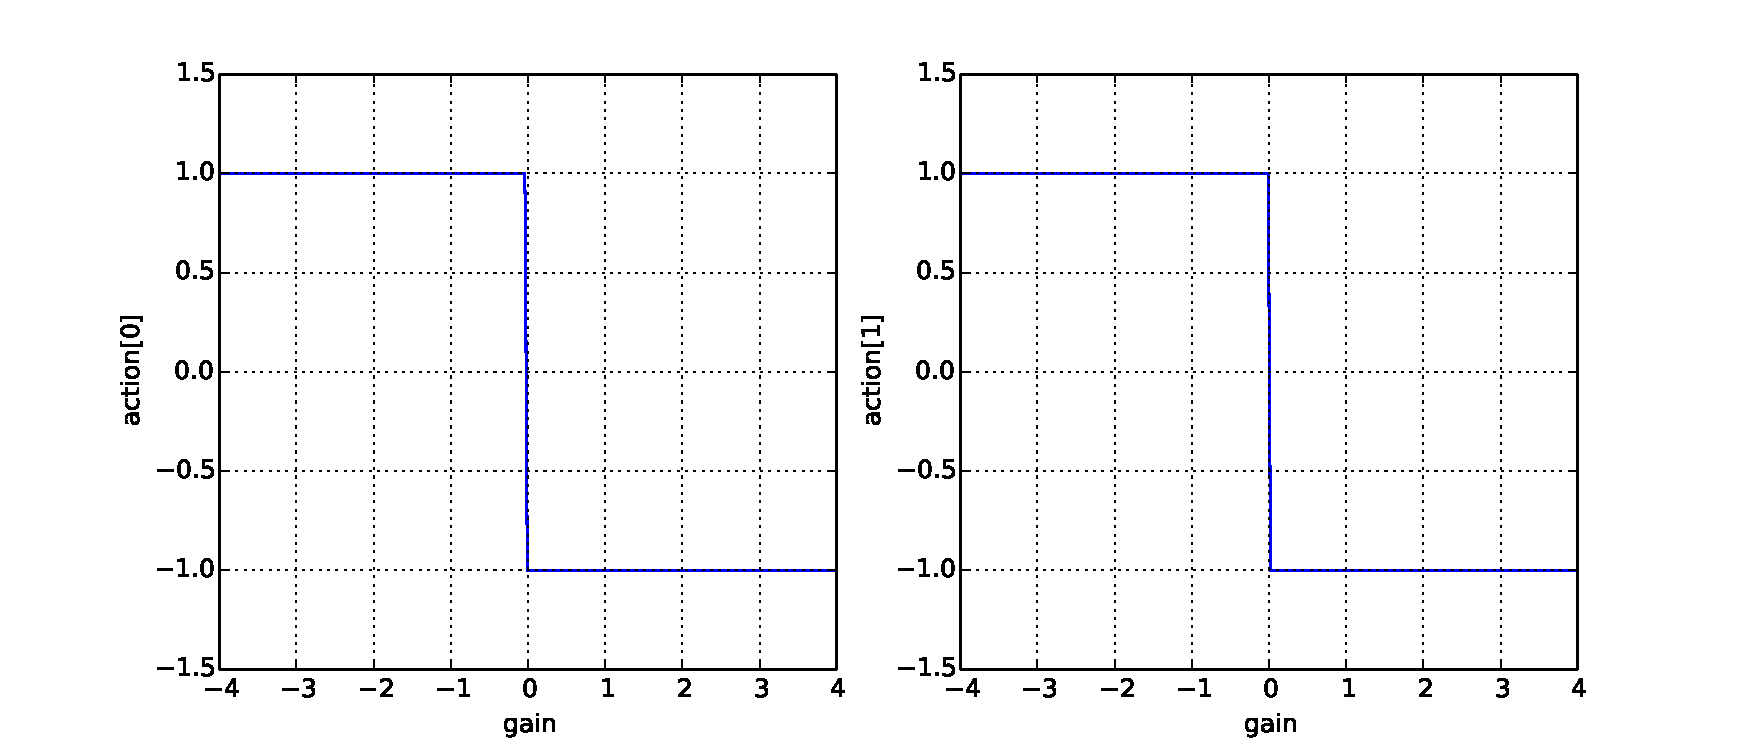
\includegraphics[width=0.85 \textwidth]{pointmass_conditional_action.pdf}
\caption{
Action of trained \embed{} policy at initial state (position $ = (1,1)$, velocity $=(0,0)$) conditioned on gain factor $g$.
Outputs are clipped to valid action range.
Plots show that policy has learned the optimal bang-bang control policy in both positive and negative gain scenarios.
\TODO{condense into fig. 2.}
}
\label{fig:conditional_action}
\end{figure}
\end{comment}



\section{Experimental details}
\label{appendix-exp}
\begin{comment}
\begin{figure}[ht]
\centering
\textbf{Training Time:}

\vspace{0.4cm}
\begin{tikzpicture}[scale=0.8, every node/.style={scale=0.85}]
\tikzstyle{box}=[draw=black, fill=white, inner sep=2mm, rounded corners=1mm]
\tikzstyle{bigbox}=[box, minimum height=1.6cm]
\tikzstyle{branch}=[circle,inner sep=0pt, minimum size=0.15cm, fill=black]
\tikzstyle{arrow}=[->]

\node[bigbox, align=center] (enviro) {Simulation \\ Environment};
\node[bigbox, align=center, right=1.75cm of enviro] (policy) {Policy \\ $\pi$};
\node[box, below=of enviro.south east, xshift=0.3cm] (embedder) {Embedder $\embedfn$};
\node[box, right=of policy, align=center] (traj)
{
  Trajectory $\tau$ \\
  \begin{tikzpicture}
  \foreach \offset in {1,...,5}
  {
    \node[box, sharp corners] (\offset) at (-0.05 * \offset, 0.1 * \offset) {$s_{t - 1},\ a_{t-1}$};
  }
  \end{tikzpicture}
};
\node[box, right=of traj] (estimator) {Estimator $\idfn$};
\node[box, below=0.65cm of traj, align=center] (sup-loss) {Supervised\\ Learning Loss};

\draw [arrow] ([yshift=0.4cm]enviro.east) -- node [above] {states} ([yshift=0.4cm]policy.west);
\draw [arrow] ([yshift=-0.4cm]policy.west) -- node [below] {actions} ([yshift=-0.4cm]enviro.east);
\draw [arrow] ([xshift=-0.5cm]enviro.south) |- node [pos=0.25, right] {SysID} (embedder.west);
\draw [arrow] (embedder.east) -| node [branch, label=below:{embeddings}] (embeds) {} (policy.south);
\draw [arrow] (traj) -- (estimator);
\draw [arrow] ([xshift=0.5cm]estimator.south) |- node [pos=0.35, left, align=right] {estimated\\embeddings} (embeds-|sup-loss.east);
\draw [arrow] (embeds) -- (embeds-|sup-loss.west);
\end{tikzpicture}

\vspace{0.8cm}

\textbf{Testing Time:}

\vspace{0.4cm}
\begin{tikzpicture}[scale=0.8, every node/.style={scale=0.85}]
\tikzstyle{box}=[draw=black, fill=white, inner sep=2mm, rounded corners=1mm]
\tikzstyle{bigbox}=[box, minimum height=1.6cm]
\tikzstyle{branch}=[circle,inner sep=0pt, minimum size=0.15cm, fill=black]
\tikzstyle{arrow}=[->]

\node[bigbox, align=center] (enviro) {Test \\ Environment};
\node[bigbox, align=center, right=1.75cm of enviro] (policy) {Policy \\ $\pi$};
\node[below=1.2cm of enviro.south east, xshift=-0.75cm, text=red, inner sep=0pt] (embedder) {$\times$};
\node[box, right=of policy, align=center] (traj)
{
  Trajectory $\tau$ \\
  \begin{tikzpicture}
  \foreach \offset in {1,...,5}
  {
    \node[box, sharp corners] (\offset) at (-0.05 * \offset, 0.1 * \offset) {$s_{t - 1},\ a_{t-1}$};
  }
  \end{tikzpicture}
};
\node[box, right=of traj] (estimator) {Estimator $\idfn$};
%\node[below=0.65cm of traj, align=center] (est-embed) {estimated\\ embeddings};

\draw [arrow] ([yshift=0.4cm]enviro.east) -- node [above] {states} ([yshift=0.4cm]policy.west);
\draw [arrow] ([yshift=-0.4cm]policy.west) -- node [below] {actions} ([yshift=-0.4cm]enviro.east);
\draw [draw=red, text=red] ([xshift=-0.5cm]enviro.south) |- node [pos=0.25, right] {SysID} (embedder.west);
%\draw [arrow] (embedder.east) -| node [branch, label=below:{embeddings}] (embeds) {} (policy.south);
\draw [arrow] (traj) -- (estimator);

%\draw [arrow] ([xshift=0.5cm]estimator.south) |- (est-embed);
%\draw [arrow] (est-embed) -| (policy.south);
\draw [arrow, draw=blue, text=blue] ([xshift=0.5cm]estimator.south) |- ++(0,-1.85cm) node [below=0.35cm of traj, align=center]{estimated\\embeddings}  -| (policy.south);

%\draw [arrow] (embeds) -- (embeds-|sup-loss.west);
\end{tikzpicture}

\vspace{0.4cm}
\caption{
Overview of our experimental setup.
At training time, correct dynamics parameters are available from the simulator.
A mapping $\embedfn$ from parameters to an abstract embedding space is learned,
along with a module $\idfn$ to identify the embedding value from a state-action trajectory $\tau$.
The policy is rewarded for behavior that improves system identification accuracy.
At testing time, the true dynamics parameters are no longer known,
and the estimated embeddings are input directly to the policy.
}
\label{fig:overview}
\end{figure}
\end{comment}

\subsection{Policy and identifier parameterizations}
In our experiments,
the policy $\pi_\latvar$ is parameterized as a fully connected neural network
with 2 hidden layers of 128 units each, using ReLU nonlinearities~\cite{nair-ReLU}.
%The advantage function used as a baseline by PPO uses an identical network.
The same architecture is used to parameterize the value- and $Q$-function estimators used by SAC.
The embedding function $\embedfn$ network contains one hidden layer of 128 units.
%We observed that parameterizing $\pi$ with a larger fully connected network significantly improved rewards
%compared to our initial choice of a $2 \times 128$ network, which can achieve very high rewards on the standard half-cheetah environment.
%This suggests that the embedding-conditioned policy learns a significantly more complex function than what is needed for a fixed-dynamics environment.

We employ a one-dimensional convolutional architecture for the identifier function $\idfn$,
composed of three 1D-convolutional layers, each with 64 filters of width 3 and ReLU activation,
followed by a single fully connected layer with 128 units, and a linear output layer.
The convolutional architecture is chosen to allow a longer trajectory window $K$ without requiring a large number of parameters
($K = 16$ in our experiments).
Additionally, it matches the intuition that differentiation and/or integration of the state and action trajectories
is often required to identify the underlying dynamics parameters.
For example, an engineered approach for estimating the gain parameter of the point-mass environment could differentiate the velocity observation to obtain acceleration.

\subsection{RL algorithm}
For all experiments, we use the entropy-regularized Soft Actor-Critic (SAC) reinforcement learning algorithm~\citep{haarnoja-soft-actor-critic}.
SAC is an off-policy algorithm where a stochastic policy is trained only with TD-learned value function estimates.
We observed significantly higher rewards using SAC compared to the on-policy, Monte Carlo policy gradient algorithm PPO~\cite{schulman-ppo}.
We conjecture that the use of TD-learning and a replay buffer is especially helpful in our scenario compared to single-environment training,
since the replay buffer helps prevent ``forgetting'' about areas of the dynamics distribution $\idpdf$ that have not been sampled recently.

The value function estimators used by SAC are parameterized by fully-connected networks of identical structure to the policy.
For \blind{} policies, the value function networks are conditioned only on the observed state $\obvar \in \obset$ to emulate domain randomization approaches.
For \plain{} policies, they are conditioned on both $\obvar$ and $\idvar \in \idset$ to emulate the setup of~\citep{yu-up-osi-rss17}.
For \embed{} policies, they are conditioned on $\obvar$, $\idvar$, and $\latvar \in \latset$.
The gradient update of the embedding function $\embedfn$ is only taken w.r.t. the policy reward and not the value function training losses.



\subsection{Randomized Half-Cheetah environment}

\begin{figure}[ht]
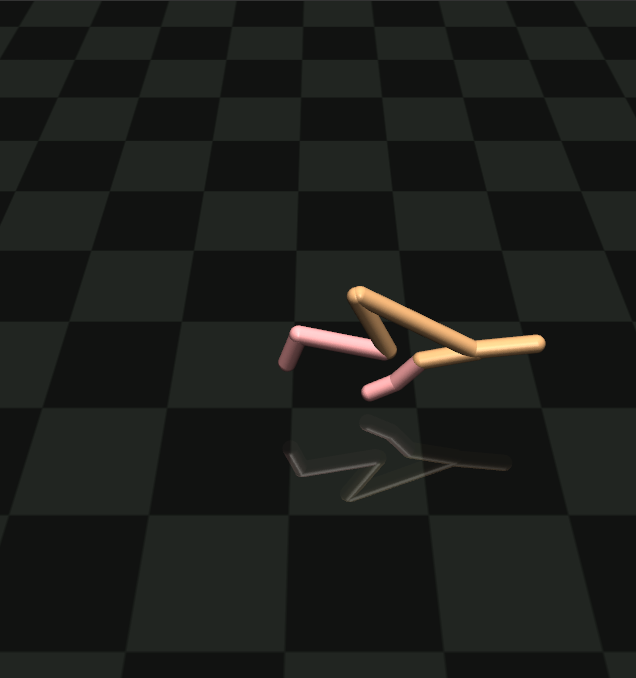
\includegraphics[trim=4cm 3cm 0cm 4cm, clip, width=0.22\textwidth]{cheetah_short.png}\hfill
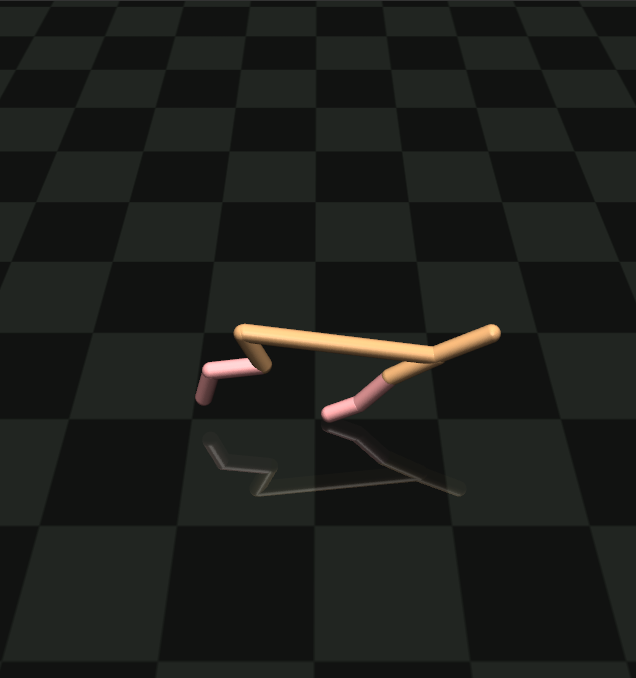
\includegraphics[trim=4cm 3cm 0cm 4cm, clip, width=0.22\textwidth]{cheetah_medium.png}\hfill
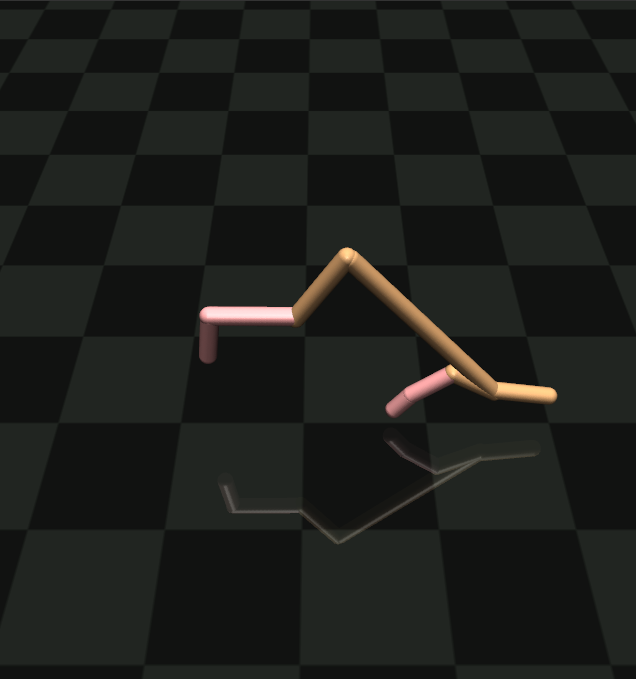
\includegraphics[trim=4cm 3cm 0cm 4cm, clip, width=0.22\textwidth]{cheetah_backleg.png}\hfill
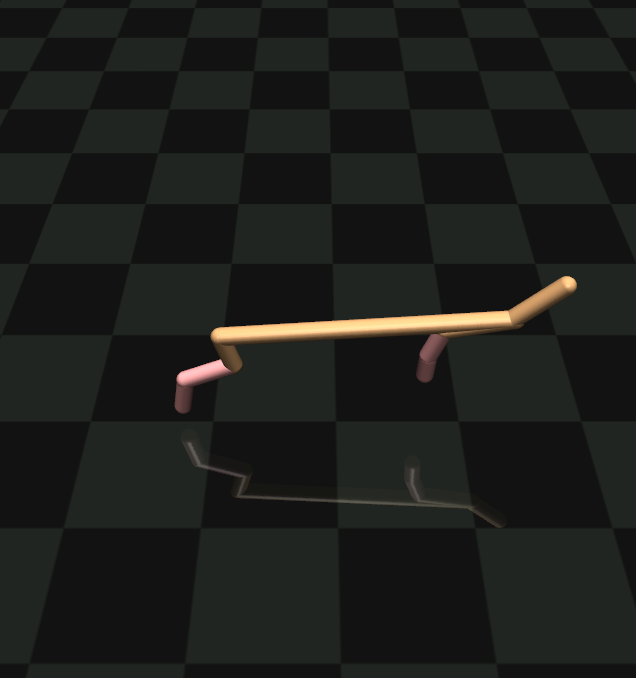
\includegraphics[trim=4cm 3cm 0cm 4cm, clip, width=0.22\textwidth]{cheetah_long.png}
\caption{Variations of Half-Cheetah environment produced by randomization of kinematic and dynamic properties.}
\label{cheetahs}
\end{figure}

Here we give more details on our procedure for randomizing the Half-Cheetah environment.
The following parameters are randomized:
lengths of seven kinematic links,
damping, stiffness~\footnote{Joint stiffness in MuJoCo denotes the strength of a virtual spring pulling the joint to its resting position.}, and ranges of six planar revolute joints,
and gear ratios of six rotary actuators.
In total, 37 parameters are randomized.
For joint ranges, limits on either side are shifted by $\omega \sim \unif(-0.3, 0.3)$ radians.
All other parameters must take nonnegative values, and some should not be too close to zero.
Thus, we multiply those parameters by a random nonnegative ratio $\beta^p$ where $p \sim \unif(-1, 1)$.
The parameter $\beta > 1$ controls the amount of randomness.
For example, if $\beta = 2$, then $ 1/2 \leq \beta^p \leq 2$.
In our experiments, $\beta = 1.75$, which was the largest value we could use without generating too many overly difficult configurations.
Some examples of the randomized half-cheetahs are shown in~\Cref{cheetahs}.

Due to the architecture of the MuJoCo physics simulator used in this environment~\citep{todorov-mujoco},
it is not practical to sample new random dynamics parameters $\idvar$ for each training iteration.
Instead, we construct a ``universe'' of 256 models initially, and sample a new ``universe'' at test time.



\end{document}
